\documentclass[tikz,border=3pt]{standalone}
\usepackage[utf8]{inputenc}
\usepackage[T1]{fontenc}
\usepackage{lmodern}
\renewcommand{\familydefault}{\sfdefault}
\usepackage{sansmath}\sansmath
\usepackage{chemfig}
\usepackage{pgfplots}\pgfplotsset{compat=1.18,/pgf/number format/use comma,/pgf/number format/1000 sep={.}}
\usetikzlibrary{arrows.meta,calc,positioning,decorations.pathmorphing,patterns}
% paleta del sitio
\definecolor{nar}{HTML}{E8680C}\definecolor{narc}{HTML}{FFB35C}\definecolor{hielo}{HTML}{FFF3E8}
\definecolor{tinta}{HTML}{1D1D1F}\definecolor{gris}{HTML}{6E6E73}\definecolor{lila}{HTML}{7C5CF0}
\definecolor{azul}{HTML}{2F6FD6}\definecolor{menta}{HTML}{17A673}\definecolor{coral}{HTML}{E8342A}
\begin{document}
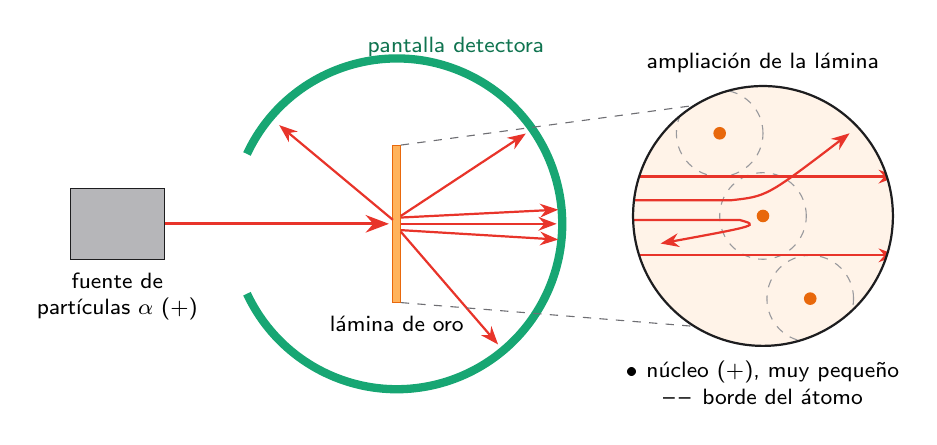
\begin{tikzpicture}[font=\small]

\fill[gris!50,draw=tinta] (-1.5,-0.45) rectangle (-0.3,0.45);
\node[anchor=north,align=center,font=\footnotesize] at (-0.9,-0.5) {fuente de\\partículas $\alpha$ (+)};
\draw[coral,very thick,-{Stealth}] (-0.3,0) -- (2.55,0);
\draw[menta,line width=3pt] (2.65,0) ++(155:2.1) arc (155:-155:2.1);
\node[anchor=south,font=\footnotesize,text=menta!70!black] at (3.4,2.0) {pantalla detectora};
\fill[narc,draw=nar] (2.6,-1.0) rectangle (2.7,1.0);
\node[anchor=north,font=\footnotesize] at (2.65,-1.05) {lámina de oro};
\draw[coral,thick,-{Stealth}] (2.7,0) -- (4.68,0);
\draw[coral,thick,-{Stealth}] (2.7,0.08) -- (4.7,0.18);
\draw[coral,thick,-{Stealth}] (2.7,-0.08) -- (4.7,-0.2);
\draw[coral,thick,-{Stealth}] (2.7,0.1) -- ($(2.65,0)+(35:2.0)$);
\draw[coral,thick,-{Stealth}] (2.7,-0.1) -- ($(2.65,0)+(-50:2.0)$);
\draw[coral,thick,-{Stealth}] (2.6,0.05) -- ($(2.65,0)+(140:1.95)$);
\draw[gris,dashed] (2.7,1.0) -- (6.4,1.5); \draw[gris,dashed] (2.7,-1.0) -- (6.4,-1.3);
\begin{scope}\clip (7.3,0.1) circle (1.65);
\fill[hielo] (7.3,0.1) circle (1.65);
\draw[gris!70,dashed] (7.3,0.1) circle (0.55);
\draw[gris!70,dashed] (6.75,1.15) circle (0.55);
\draw[gris!70,dashed] (7.9,-0.95) circle (0.55);
\draw[coral,thick,-{Stealth}] (5.6,0.6) -- (9,0.6);
\draw[coral,thick,-{Stealth}] (5.6,-0.4) -- (9,-0.4);
\draw[coral,thick,-{Stealth}] (5.6,0.3) -- (6.9,0.3) .. controls (7.35,0.35) .. (8.4,1.15);
\draw[coral,thick,-{Stealth}] (5.6,0.05) -- (7,0.05) .. controls (7.25,-0.02) .. (6,-0.25);
\fill[nar] (7.3,0.1) circle (0.08);
\fill[nar] (6.75,1.15) circle (0.08);
\fill[nar] (7.9,-0.95) circle (0.08);
\end{scope}
\draw[tinta,thick] (7.3,0.1) circle (1.65);
\node[anchor=south,font=\footnotesize] at (7.3,1.8) {ampliación de la lámina};
\node[anchor=north,align=center,font=\footnotesize] at (7.3,-1.62) {\textbullet\ núcleo (+), muy pequeño\\--\,--\, borde del átomo};

\end{tikzpicture}
\end{document}
